\documentclass[]{article}

\usepackage[margin=2cm]{geometry}
\usepackage{graphicx} % Allows including images
\usepackage{booktabs} % Allows the use of \toprule, \midrule and \bottomrule in tables
\usepackage{textcomp}
\usepackage{threeparttable}
\usepackage{tikz}
\usepackage[utf8]{inputenc}
\usepackage{makecell}
\usepackage{marvosym}
\usepackage{eurosym}
\usepackage{threeparttablex}
\usepackage{tabularx}
\usepackage{subcaption} % For subfigures with captions
\usepackage{float} % Provides the [H] placement option
\DeclareUnicodeCharacter{20AC}{\EUR{}}
\usepackage[normalem]{ulem}

%opening
\title{`Family Risk Sharing'\\`When the Shock Hits the Knot: Individual Consumption Insurance Among Spouses'\\`When the Shock Hits the Knot: bargaining and family risk sharing'}

\author{B-C-V}

\begin{document}

\maketitle

\section{Summary statistics and life-cycle behavior}

%Summary statistics
\begin{table}[h]\centering
	
	\caption{Summary statistics}
	\label{table:sum_stat}
	\begin{threeparttable}[t]\centering
		\begin{tabular*}{\textwidth}{l@{\extracolsep{\textwidth minus \textwidth}}ccccc}
			\toprule
			& Household& Household  & Wife, Private & Husband, Private & Home good  \\
        	& assets  & earnings  & consumption & consumption & expenditure  \\[0.5ex]			&  (1)& (2) & (3) & (4) & (5)   \\[0.5ex]
			\midrule		
			Mean wrt mean earnings          & 6.487 & 1.996 & 0.155 & 0.310 & 1.839    \\ Gini          & 0.650 & 0.472 & 0.530 & 0.404 & 0.303    \\ Top 1\% share & 0.074 & 0.050 & 0.070 & 0.043 & 0.032    \\\bottomrule    
			\\[-2.5ex] 
		\end{tabular*}
		\begin{tablenotes}[flushleft]
			\footnotesize{\item \textsc{Notes}: assets and earnings are measure across the population regardless of marital status, while other variables are measured among married households.
			}
		\end{tablenotes}
	\end{threeparttable}
\end{table}


%Life-cycle behavior
\begin{figure}[H]
	\centering
	% First picture
	\begin{subfigure}{0.49\textwidth} % Adjust width as needed
		\centering
		\includegraphics[width=\textwidth]{lifecycle_aggregate.eps} % Replace with your first pgf file name
		\caption{Married couples + single women}
		\label{fig:picture1}
	\end{subfigure}
	% Second picture
	\begin{subfigure}{0.49\textwidth}
		\centering
		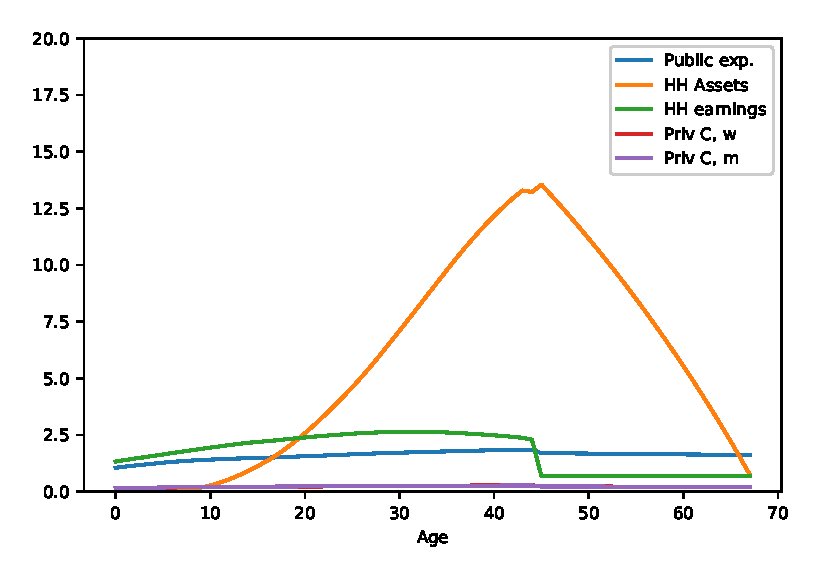
\includegraphics[width=\textwidth]{lifecycle_married.eps} % Replace with your second pgf file name
		\caption{Married couples}
		\label{fig:picture2}
	\end{subfigure}
	% Third picture
	\begin{subfigure}{0.49\textwidth}
		\centering
		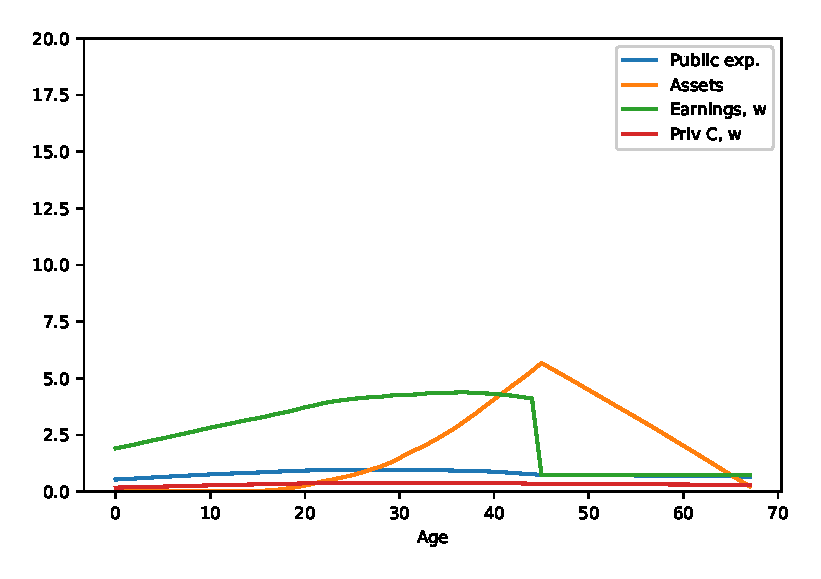
\includegraphics[width=\textwidth]{lifecycle_singlew.eps} % Replace with your third pgf file name
		\caption{Single women}
		\label{fig:picture3}
	\end{subfigure}
	
	\caption{Life-cycle behavior of different types of household, averages}
	\label{fig:all_pictures}
\end{figure}

\section{Log consumption and income growth}

\begin{table}[h]\centering
	
	\caption{Moments of the log growth of the variables reported in the rows}
	\label{table:log_growth_moments}
	\begin{threeparttable}[t]\centering
		\begin{tabular*}{\textwidth}{l@{\extracolsep{\textwidth minus \textwidth}}cccc}
			\toprule
			& Mean & Variance  & Skeweness & Kurtosis   \\[0.5ex]
			\midrule		
			Wife, private consumption          & 0.007 & 0.017 & -4.436 & 112.704    \\ Husband, private consumption       & 0.011 & 0.013 & -1.467 & 10.547    \\ Wife share of private consumption  & -0.004 & 0.013 & -9.768 & 575.752    \\ Home good expenditure              & 0.010 & 0.005 & 0.073 & 11.077    \\ Total consumption                  & 0.010 & 0.006 & 0.017 & 10.547    \\ Wife, earnings                     & 0.007 & 0.040 & -3.268 & 37.644    \\ Husband, earnings                  & 0.012 & 0.025 & 0.009 & 3.573    \\\bottomrule    
			\\[-2.5ex] 
		\end{tabular*}
		\begin{tablenotes}[flushleft]
			\footnotesize{\item \textsc{Notes}: sample of those who stay married over two consecutive periods.
			}
		\end{tablenotes}
	\end{threeparttable}
\end{table}


%Life-cycle behavior
\begin{figure}[H]
	\centering
	% First picture
	\begin{subfigure}{0.49\textwidth} % Adjust width as needed
		\centering
		\includegraphics[width=\textwidth]{lifecycle_ineq1.eps} % Replace with your first pgf file name
		\label{fig:picture1}
	\end{subfigure}
	% Second picture
	\begin{subfigure}{0.49\textwidth}
		\centering
		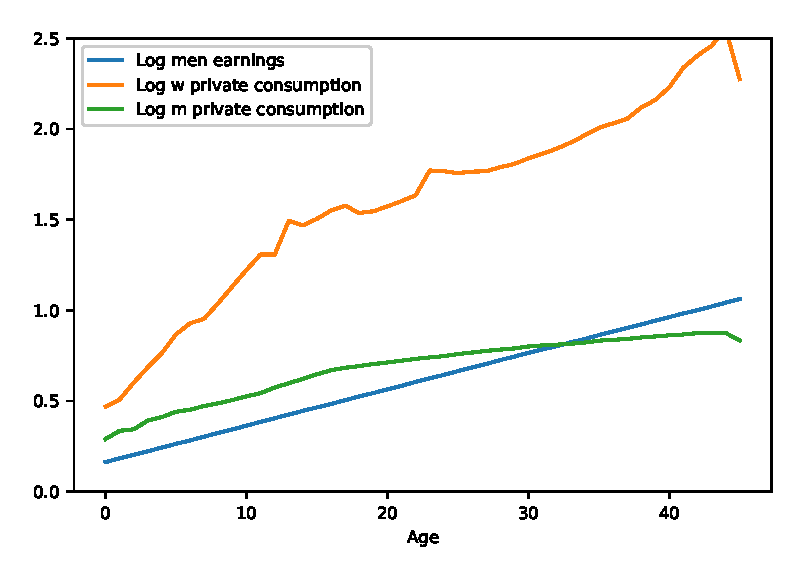
\includegraphics[width=\textwidth]{lifecycle_ineq2.eps} % Replace with your second pgf file name
		\label{fig:picture2}
	\end{subfigure}

	\caption{Variance of log earnings and consumption by age}
	\label{fig:all_pictures}
\end{figure}

\section{Marital surplus, renegotiation and divorce}

% distribution of marital surplus



%Marital surplus, renegotiations and divorce

\begin{figure}[H]
	\centering
	% First picture
	\begin{subfigure}{0.49\textwidth} % Adjust width as needed
		\centering
		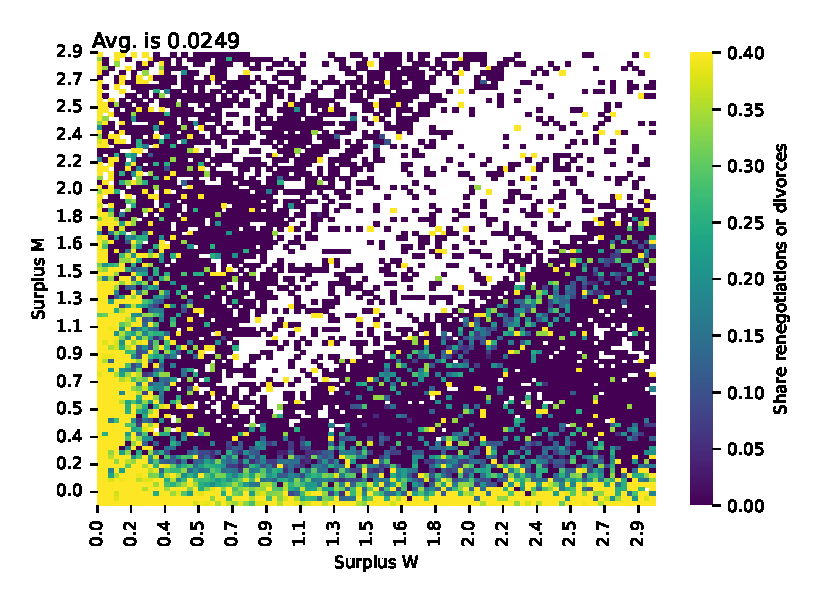
\includegraphics[width=\textwidth]{surp_ren_div.eps} % Replace with your first pgf file name
		\caption{Renegotiations and divorces}
		\label{fig:picture1}
	\end{subfigure}
	% Second picture
	\begin{subfigure}{0.49\textwidth}
		\centering
		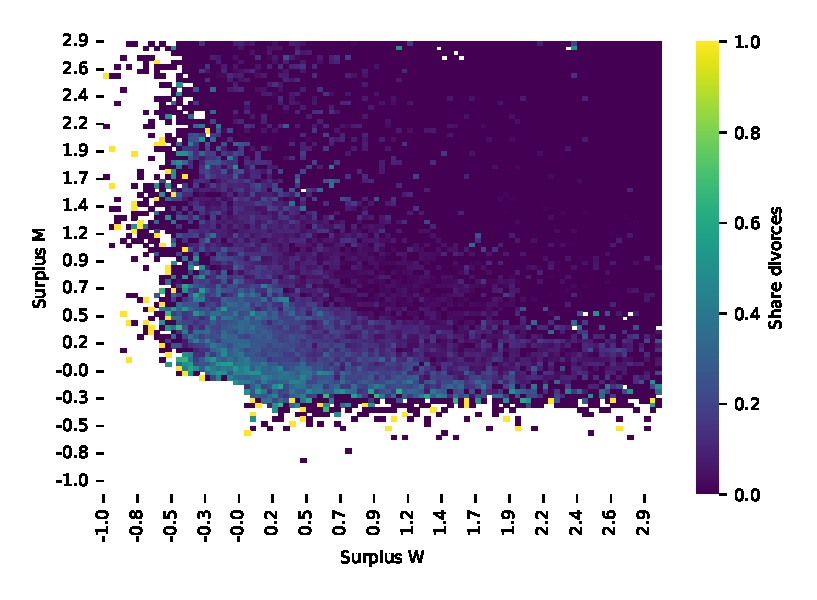
\includegraphics[width=\textwidth]{surp_div.eps} % Replace with your second pgf file name
		\caption{Divorces}
		\label{fig:picture2}
	\end{subfigure}
	% Third picture
	\begin{subfigure}{0.49\textwidth}
		\centering
		\includegraphics[width=\textwidth]{surp_renw.eps} % Replace with your third pgf file name
		\caption{Renegotiations triggered by the wife}
		\label{fig:picture3}
	\end{subfigure}
		% Third picture
	\begin{subfigure}{0.49\textwidth}
		\centering
		\includegraphics[width=\textwidth]{surp_renm.eps} % Replace with your third pgf file name
		\caption{Renegotiation triggered by the husband}
		\label{fig:picture3}
	\end{subfigure}
	
	\caption{Marital surplus, renegotiation and divorce}
	\label{fig:surp_ren}
\end{figure}


% distribution of marital surplus
\begin{figure}[H]
	\centering
	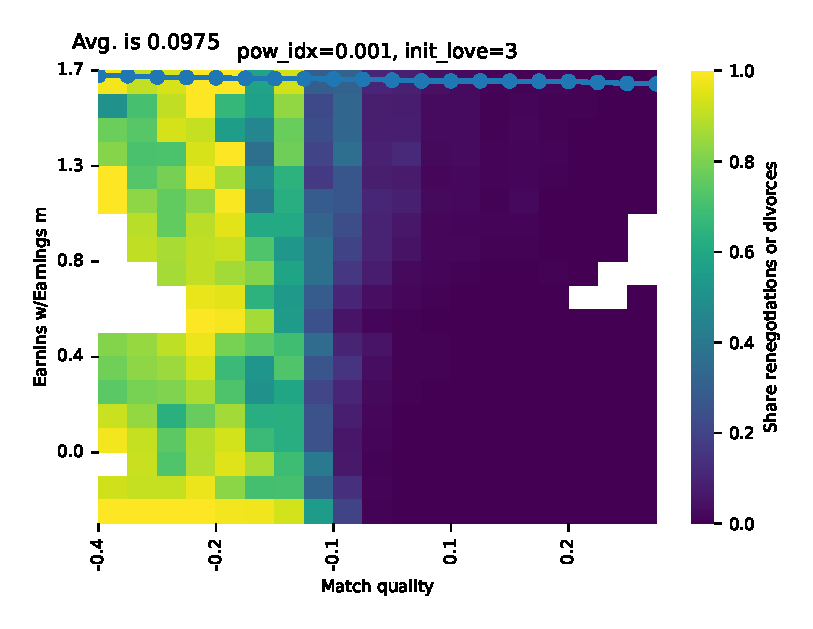
\includegraphics[width=\textwidth]{match_earn_ren_div.eps} 
	\caption{Share or divorces and renegotiations given relative earnings and match quality}
	\label{fig:surplus match earn}
\end{figure}


%Marital surplus and shocks to 

\begin{figure}[H]
	\centering
	% First picture
	\begin{subfigure}{0.49\textwidth} % Adjust width as needed
		\centering
		\includegraphics[width=\textwidth]{shocks_ren_div.eps} % Replace with your first pgf file name
		\caption{Renegotiations and divorces}
		\label{fig:picture1}
	\end{subfigure}
	% Second picture
	\begin{subfigure}{0.49\textwidth}
		\centering
		\includegraphics[width=\textwidth]{shocks_div.eps} % Replace with your second pgf file name
		\caption{Divorces}
		\label{fig:picture2}
	\end{subfigure}
	% Third picture
	\begin{subfigure}{0.49\textwidth}
		\centering
		\includegraphics[width=\textwidth]{shocks_ren_w.eps} % Replace with your third pgf file name
		\caption{Renegotiations triggered by the wife}
		\label{fig:picture3}
	\end{subfigure}
	% Third picture
	\begin{subfigure}{0.49\textwidth}
		\centering
		\includegraphics[width=\textwidth]{shocks_ren_m.eps} % Replace with your third pgf file name
		\caption{Renegotiation triggered by the husband}
		\label{fig:picture3}
	\end{subfigure}
	
	\caption{M and W income shocks, renegotiation and divorce}
	\label{fig:surp_ren}
\end{figure}

%Distribution of marital surplus

\begin{figure}[H]
	\centering
	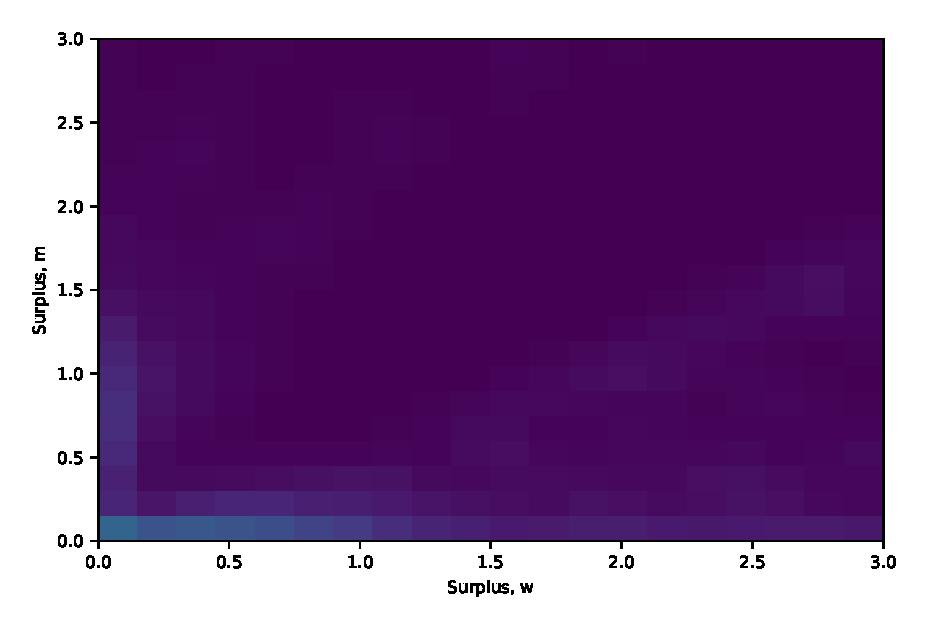
\includegraphics[width=\textwidth]{surplus_dist.eps} 
	\caption{Marital surplus distribution (value of staying married - value of divorce)}
	\label{fig:surplus dist}
\end{figure}



\begin{figure}[H]
	\centering
	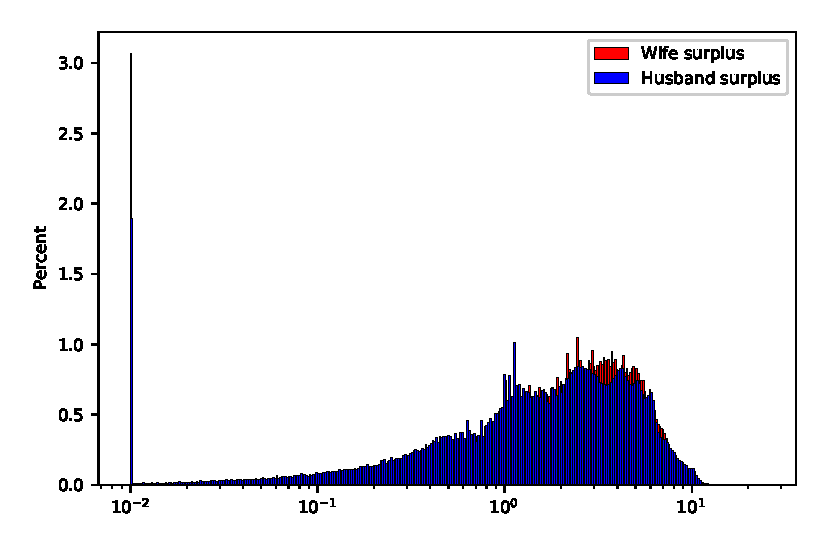
\includegraphics[width=\textwidth]{surplus_dist_2d.eps} 
	\caption{Marital surplus distribution}
	\label{fig:surplus dist_2d}
\end{figure}


\begin{figure}[H]
	\centering
	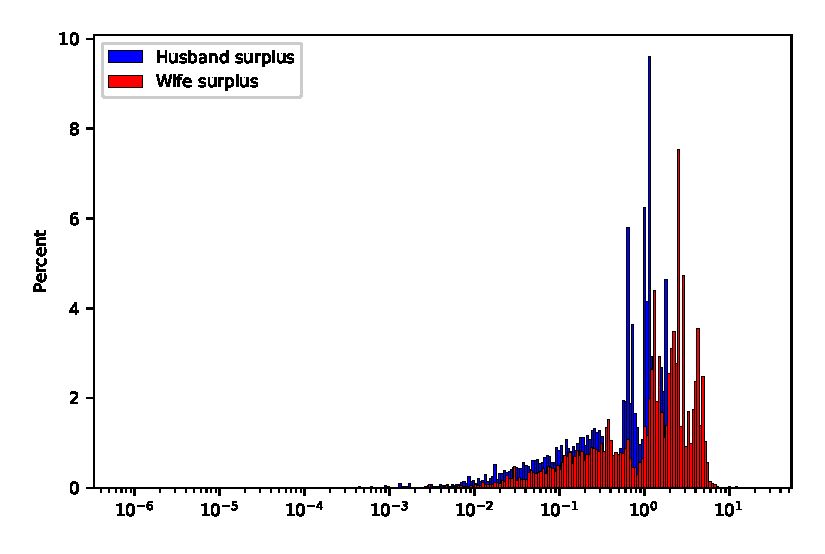
\includegraphics[width=\textwidth]{surplus_dist_i_2d.eps} 
	\caption{Marital surplus distribution at meeting}
	\label{fig:surplus dist_i_2d}
\end{figure}


Something we have learned
\begin{itemize}
	\item The match surplus at meeting is higher for women (Figure \ref{fig:surplus dist_i_2d}): this is an implication of the (close to) symmetric nash bargaining (SNB) and women earning less than men. SNB allocates a higher share of the surplus to the spouse having lower earnings. 
	\item Women are more likely to hit the participation constraint than men (Figure \ref{fig:surplus dist_2d}). Since, again, women's marginal utility is higher than for men, the same shock implies a larger change in reservation utilities for women than for men.
	\item If we impose a non-symmetric nash bargaining, the gender who gets a higher weight will be less likely to hit participation constraints.
	\item If we close the gender wage gap, the patterns in renegotiation and surplus share distribution become gender symmetric
	
	\item To be checked with the policy experiment how labor supply is reacting. If, when outside option for women improve, labor supply goes down, our model cannot replicate it. 
	
	\item Excess kurtosis of women consumption seems to be driven by renegotiations 
\end{itemize}

\section{Consumption insurance regressions}
%%%%%%%%%%%%%%%%%%%%%%%%
%All income
%%%%%%%%%%%%%%%%%%%%%%%
\begin{table}[h]\centering
	
	\caption{Pass-through of changes in income on consumption and consumption shares, using changes in...}
	\label{table:allinc}
	\begin{threeparttable}[t]\centering
		\begin{tabular*}{\textwidth}{l@{\extracolsep{\textwidth minus \textwidth}}ccccc}
			\toprule
			& Total Exp  & Common Exp  & Husband Exp & Wife Exp & Wife share  \\[0.5ex]
			&  (1)& (2) & (3) & (4) & (5)   \\[0.5ex]
			\midrule		
			...total income   & \textbf{0.309} & 0.276 & & &    \\ ...wife income    & 0.080 & 0.077&  \textbf{0.092} &  \textbf{0.096} &  \textbf{0.004}    \\ ...husband income & 0.177 &  0.172&  \textbf{0.204} &  \textbf{0.179} &  \textbf{-0.025}    \\\bottomrule    
			\\[-2.5ex] 
		\end{tabular*}
		\begin{tablenotes}[flushleft]
			\footnotesize{\item \textsc{Notes}: Coefficient interpretation: 1\% change in income leads to X\% change in expenditure. Coefficients associated to changes in the wife income are computed using women working in two consecutive periods.
			}
		\end{tablenotes}
	\end{threeparttable}
\end{table}



%%%%%%%%%%%%%%%%%%%%%%%%
%Transitory income changes
%%%%%%%%%%%%%%%%%%%%%%%
\begin{table}[h]\centering
	
	\caption{Pass-through of changes in income on consumption and consumption shares, using \textbf{transitory
		} changes in...}
	\label{table:trainc}
	\begin{threeparttable}[t]\centering
		\begin{tabular*}{\textwidth}{l@{\extracolsep{\textwidth minus \textwidth}}ccccc}
			\toprule
			& Total Exp  & Common Exp  & Husband Exp & Wife Exp & Wife share  \\[0.5ex]
			&  (1)& (2) & (3) & (4) & (5)   \\[0.5ex]
			\midrule		
			...total income   & \textbf{0.054} & 0.051 & & &    \\ ...wife income    & 0.040 & 0.039&  \textbf{0.045} &  \textbf{0.044} &  \textbf{0.000}    \\ ...husband income & 0.054 &  0.052&  \textbf{0.072} &  \textbf{0.013} &  \textbf{-0.048}    \\\bottomrule    
			\\[-2.5ex] 
		\end{tabular*}
		\begin{tablenotes}[flushleft]
			\footnotesize{\item \textsc{Notes}: Coefficient interpretation: 1\% change in income leads to X\% change in expenditure. Coefficients associated to changes in the wife income are computed using women working in two consecutive periods.
			}
		\end{tablenotes}
	\end{threeparttable}
\end{table}

%%%%%%%%%%%%%%%%%%%%%%%%%%%
%Persistent income changes
%%%%%%%%%%%%%%%%%%%%%%%%%%
\begin{table}[h]\centering
	
	\caption{Pass-through of changes in income on consumption and consumption shares, using \textbf{persistent} changes in...}
	\label{table:persinc}
	\begin{threeparttable}[t]\centering
		\begin{tabular*}{\textwidth}{l@{\extracolsep{\textwidth minus \textwidth}}ccccc}
			\toprule
			& Total Exp  & Common Exp  & Husband Exp & Wife Exp & Wife share  \\[0.5ex]
			&  (1)& (2) & (3) & (4) & (5)   \\[0.5ex]
			\midrule		
			...total income   & \textbf{0.303} & 0.330 & & &    \\ ...wife income    & 0.127 & 0.136&  \textbf{0.033} &  \textbf{0.084} &  \textbf{0.051}    \\ ...husband income & 0.412 &  0.435&  \textbf{0.240} &  \textbf{0.226} &  \textbf{-0.014}    \\\bottomrule    
			\\[-2.5ex] 
		\end{tabular*}
		\begin{tablenotes}[flushleft]
			\footnotesize{\item \textsc{Notes}: Coefficient interpretation: 1\% change in income leads to X\% change in expenditure. Coefficients associated to changes in the wife income are computed using women working in two consecutive periods.
			}
		\end{tablenotes}
	\end{threeparttable}
\end{table}

%%%%%%%%%%%%%%%%%%%%%%%%
%BPP MPC
%%%%%%%%%%%%%%%%%%%%%%%
\begin{table}[h]\centering
	
	\caption{MPC calculated as in BPP, using transitory changes in...}
	\label{table:BPP_MPC}
	\begin{threeparttable}[t]\centering
		\begin{tabular*}{\textwidth}{l@{\extracolsep{\textwidth minus \textwidth}}cccc}
			\toprule
			& Total Exp  & Common Exp  & Husband Exp & Wife Exp  \\[0.5ex]
			&  (1)& (2) & (3) & (4)   \\[0.5ex]
			\midrule		
			...husband income & 0.039 & 0.041 & 0.044 & 0.001  \\ ...wife income    & 0.041 & 0.039 & -0.012 & 0.083  \\ ...total income   & 0.319 & 0.279 & 0.473 & 0.521  \\\bottomrule    
			\\[-2.5ex] 
		\end{tabular*}
		\begin{tablenotes}[flushleft]
			\footnotesize{\item \textsc{Notes}: the consumption insurance parameters displayed in the table are computed as $$\frac{E\left(\Delta c_t \Delta y_{t+1}\right)}{E\left(\Delta y_t \Delta y_{t+1}\right)},$$ where $y_t$ can the income of the husband, wife or the sum of the two (total). Variables $c_t$ can be the total, common, husband or wife' expenditures. Coefficients associated to changes in the wife income are computed using women working in two consecutive periods.
			}
		\end{tablenotes}
	\end{threeparttable}
\end{table}


%%%%%%%%%%%%%%%%%%%%%%%%
%BPP PERSISTENT
%%%%%%%%%%%%%%%%%%%%%%%
\begin{table}[h]\centering
	
	\caption{Consumption insurance to persistent income shocks, calculated as in BPP, using persistent changes in...}
	\label{table:BPP_PER}
	\begin{threeparttable}[t]\centering
		\begin{tabular*}{\textwidth}{l@{\extracolsep{\textwidth minus \textwidth}}cccc}
			\toprule
			& Total Exp  & Common Exp  & Husband Exp & Wife Exp  \\[0.5ex]
			&  (1)& (2) & (3) & (4)   \\[0.5ex]
			\midrule		
			...husband income & 0.364 & 0.352 & 0.426 & 0.346  \\ ...wife income    & 0.341 & 0.334 & 0.310 & 0.499  \\ ...total income   & 0.440 & 0.418 & 0.507 & 0.619  \\\bottomrule     
			\\[-2.5ex] 
		\end{tabular*}
		\begin{tablenotes}[flushleft]
			\footnotesize{\item \textsc{Notes}: the consumption insurance parameters displayed in the table are computed as $$\frac{E\left(\Delta c_t\left(\Delta y_{t-1}+\Delta y_t+\Delta y_t\right)\right)}{E\left(\Delta y_t\left(\Delta y_{t-1}+\Delta y_t+\Delta y_t\right)\right)},$$ where $y_t$ can the income of the husband, wife or the sum of the two (total). Variables $c_t$ can be the total, common, husband or wife' expenditures. Coefficients associated to changes in the wife income are computed using women working in two consecutive periods.
}
		\end{tablenotes}
	\end{threeparttable}
\end{table}

%%%%%%%%%%%%%%%%%%%%%%%%%%%%%%%%%%
%Income shocks and labor supply
%%%%%%%%%%%%%%%%%%%%%%%%%%%%%%%%%
\begin{table}[h]\centering
	
	\caption{Women's employment response (in percentage points) to different types of income shocks}
	\label{table:shocks_WLP}
	\begin{threeparttable}[t]\centering
		\begin{tabular*}{\textwidth}{@{\extracolsep{\textwidth minus \textwidth}}cccccc}
			\toprule
			  \multicolumn{2}{c}{Transitory shocks}  &  \multicolumn{2}{c}{Persistent shocks} & \multicolumn{2}{c}{Transitory+persistent shocks}   \\[0.5ex]
			
		    \cmidrule(lr){1-2}    \cmidrule(lr){3-4}  \cmidrule(lr){5-6} 
			
			
			
			 Wife  & Husband  &Wife  & Husband  & Wife  & Husband     \\[0.5ex]
			  (1)& (2) & (3) & (4) & (5)  & (6)  \\[0.5ex]
			\midrule		
			  0.337 & -0.033 & 0.403 & -0.055 & 0.358 & -0.042  \\\bottomrule     
			\\[-2.5ex] 
		\end{tabular*}
		\begin{tablenotes}[flushleft]
			\footnotesize{\item \textsc{Notes}: the income shocks relate to \textit{potential log income} $y$. In the case of women, a positive potential income shocks does not translate in more earnings if the women does not work. The numbers displayed in the table are OLS coefficients:
				
				$$\frac{E(\Delta y_t \  \Delta WLP_t)}{E(\Delta y_t)},$$
			
			where $\Delta WLP$ is the change in women's employment over two consecutive periods.
				
			}
		\end{tablenotes}
	\end{threeparttable}
\end{table}

%%%%%%%%%%%%%%%%%%%%%%%%
%Level
%%%%%%%%%%%%%%%%%%%%%%%
\begin{table}[h]\centering
	
	\caption{Pass-through of changes in income on consumption and consumption shares, using changes in...}
	\label{table:level}
	\begin{threeparttable}[t]\centering
		\begin{tabular*}{\textwidth}{l@{\extracolsep{\textwidth minus \textwidth}}ccccc}
			\toprule
			& Total Exp  & Common Exp  & Husband Exp & Wife Exp & Wife share  \\[0.5ex]
			&  (1)& (2) & (3) & (4) & (5)   \\[0.5ex]
			\midrule		
			...total income   & \textbf{0.173} & 0.116 & & &    \\ ...wife income    & 0.171 & 0.113&  \textbf{0.035} &  \textbf{0.023} &  \textbf{0.013}    \\ ...husband income & 0.152 &  0.117&  \textbf{0.025} &  \textbf{0.011} &  \textbf{-0.016}    \\\bottomrule    
			\\[-2.5ex] 
		\end{tabular*}
		\begin{tablenotes}[flushleft]
			\footnotesize{\item \textsc{Notes}: Coefficient interpretation: 1 yen change in income leads to X yen change in expenditure. 
			}
		\end{tablenotes}
	\end{threeparttable}
\end{table}
\end{document}
